\documentclass[10pt]{article}
\usepackage{tikz}
\usepackage[margin=0cm]{geometry}
\pagestyle{empty}

\begin{document}

\vspace*{\fill}
\begin{center}
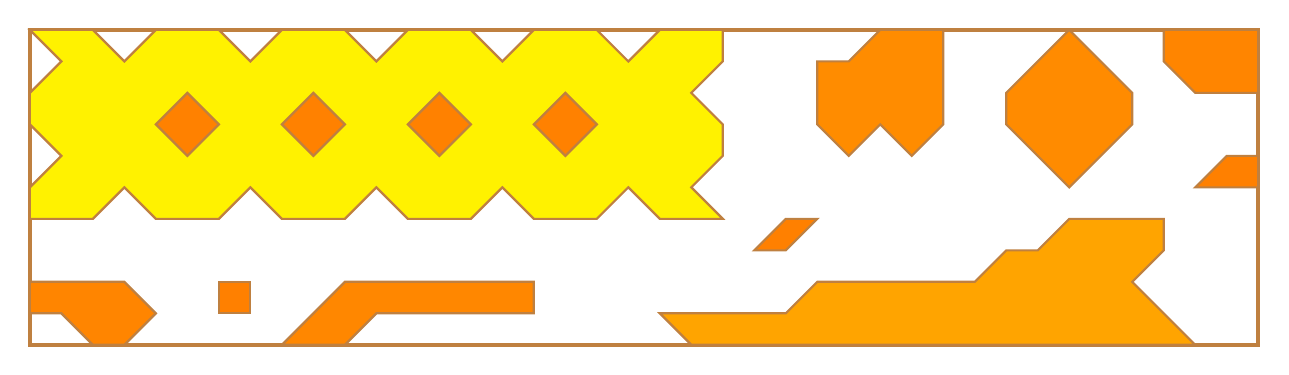
\begin{tikzpicture}[x=0.4cm, y=-0.4cm, thick, brown]
\draw[ultra thick] (0, 0) -- (39, 0) -- (39, 10) -- (0, 10) -- cycle;
%Depth 0
\filldraw[fill=orange!0!yellow] (0, 0) -- (2, 0) -- (3, 1) -- (4, 0) -- (6, 0) -- (7, 1) -- (8, 0) -- (10, 0) -- (11, 1) -- (12, 0) -- (14, 0) -- (15, 1) -- (16, 0) -- (18, 0) -- (19, 1) -- (20, 0) -- (22, 0) -- (22, 1) -- (21, 2) -- (22, 3) -- (22, 4) -- (21, 5) -- (22, 6) -- (20, 6) -- (19, 5) -- (18, 6) -- (16, 6) -- (15, 5) -- (14, 6) -- (12, 6) -- (11, 5) -- (10, 6) -- (8, 6) -- (7, 5) -- (6, 6) -- (4, 6) -- (3, 5) -- (2, 6) -- (0, 6) -- (0, 5) -- (1, 4) -- (0, 3) -- (0, 2) -- (1, 1) -- cycle;
\filldraw[fill=orange!90!yellow] (27, 0) -- (29, 0) -- (29, 3) -- (28, 4) -- (27, 3) -- (26, 4) -- (25, 3) -- (25, 1) -- (26, 1) -- cycle;
\filldraw[fill=orange!91!yellow] (33, 0) -- (35, 2) -- (35, 3) -- (33, 5) -- (31, 3) -- (31, 2) -- cycle;
\filldraw[fill=orange!96!yellow] (36, 0) -- (39, 0) -- (39, 2) -- (37, 2) -- (36, 1) -- cycle;
\filldraw[fill=orange!100!yellow] (38, 4) -- (39, 4) -- (39, 5) -- (37, 5) -- cycle;
\filldraw[fill=orange!100!yellow] (24, 6) -- (25, 6) -- (24, 7) -- (23, 7) -- cycle;
\filldraw[fill=orange!71!yellow] (33, 6) -- (36, 6) -- (36, 7) -- (35, 8) -- (37, 10) -- (21, 10) -- (20, 9) -- (24, 9) -- (25, 8) -- (30, 8) -- (31, 7) -- (32, 7) -- cycle;
\filldraw[fill=orange!96!yellow] (0, 8) -- (3, 8) -- (4, 9) -- (3, 10) -- (2, 10) -- (1, 9) -- (0, 9) -- cycle;
\filldraw[fill=orange!100!yellow] (6, 8) -- (7, 8) -- (7, 9) -- (6, 9) -- cycle;
\filldraw[fill=orange!94!yellow] (10, 8) -- (16, 8) -- (16, 9) -- (11, 9) -- (10, 10) -- (8, 10) -- cycle;
%Depth 1
\filldraw[fill=orange!99!yellow] (5, 2) -- (6, 3) -- (5, 4) -- (4, 3) -- cycle;
\filldraw[fill=orange!99!yellow] (9, 2) -- (10, 3) -- (9, 4) -- (8, 3) -- cycle;
\filldraw[fill=orange!99!yellow] (13, 2) -- (14, 3) -- (13, 4) -- (12, 3) -- cycle;
\filldraw[fill=orange!99!yellow] (17, 2) -- (18, 3) -- (17, 4) -- (16, 3) -- cycle;
\end{tikzpicture}
\end{center}
\vspace*{\fill}

\end{document}
